% !TEX root = mythesis.tex

%==============================================================================
\chapter{Extensive Air Showers}
\label{chap:EAS}
%==============================================================================

As mentioned in the previous chapter an Extensive Air Shower (EAS) is a cascade of high-energy particles that is produced when an UHECR, typically a proton or a nucleus, collides with a nucleus in Earth's atmosphere. This cascade can span over hundred to thousands of meters based on the energy of the initial particle and the incoming zenith angle. EASs offer the best way to look for UHECRs since the low flux of these particles make direct detection using detectors mounted on balloons or spacecrafts not feasible. The EAS can be detected at the ground via an array of detectors. To infer the properties of the CR from the EAS it creates, one needs to model and understand how an air shower develops in the atmosphere. This chapter describes the process of the initiation and the development of the shower induced by CRs and neutrinos. It also aims to describe the important characteristics of EASs which help in extracting the relevant information and the last part of this chapter is devoted to summarise the detection of the EASs using different detector systems. 

\begin{figure}[t!]
    \centering
    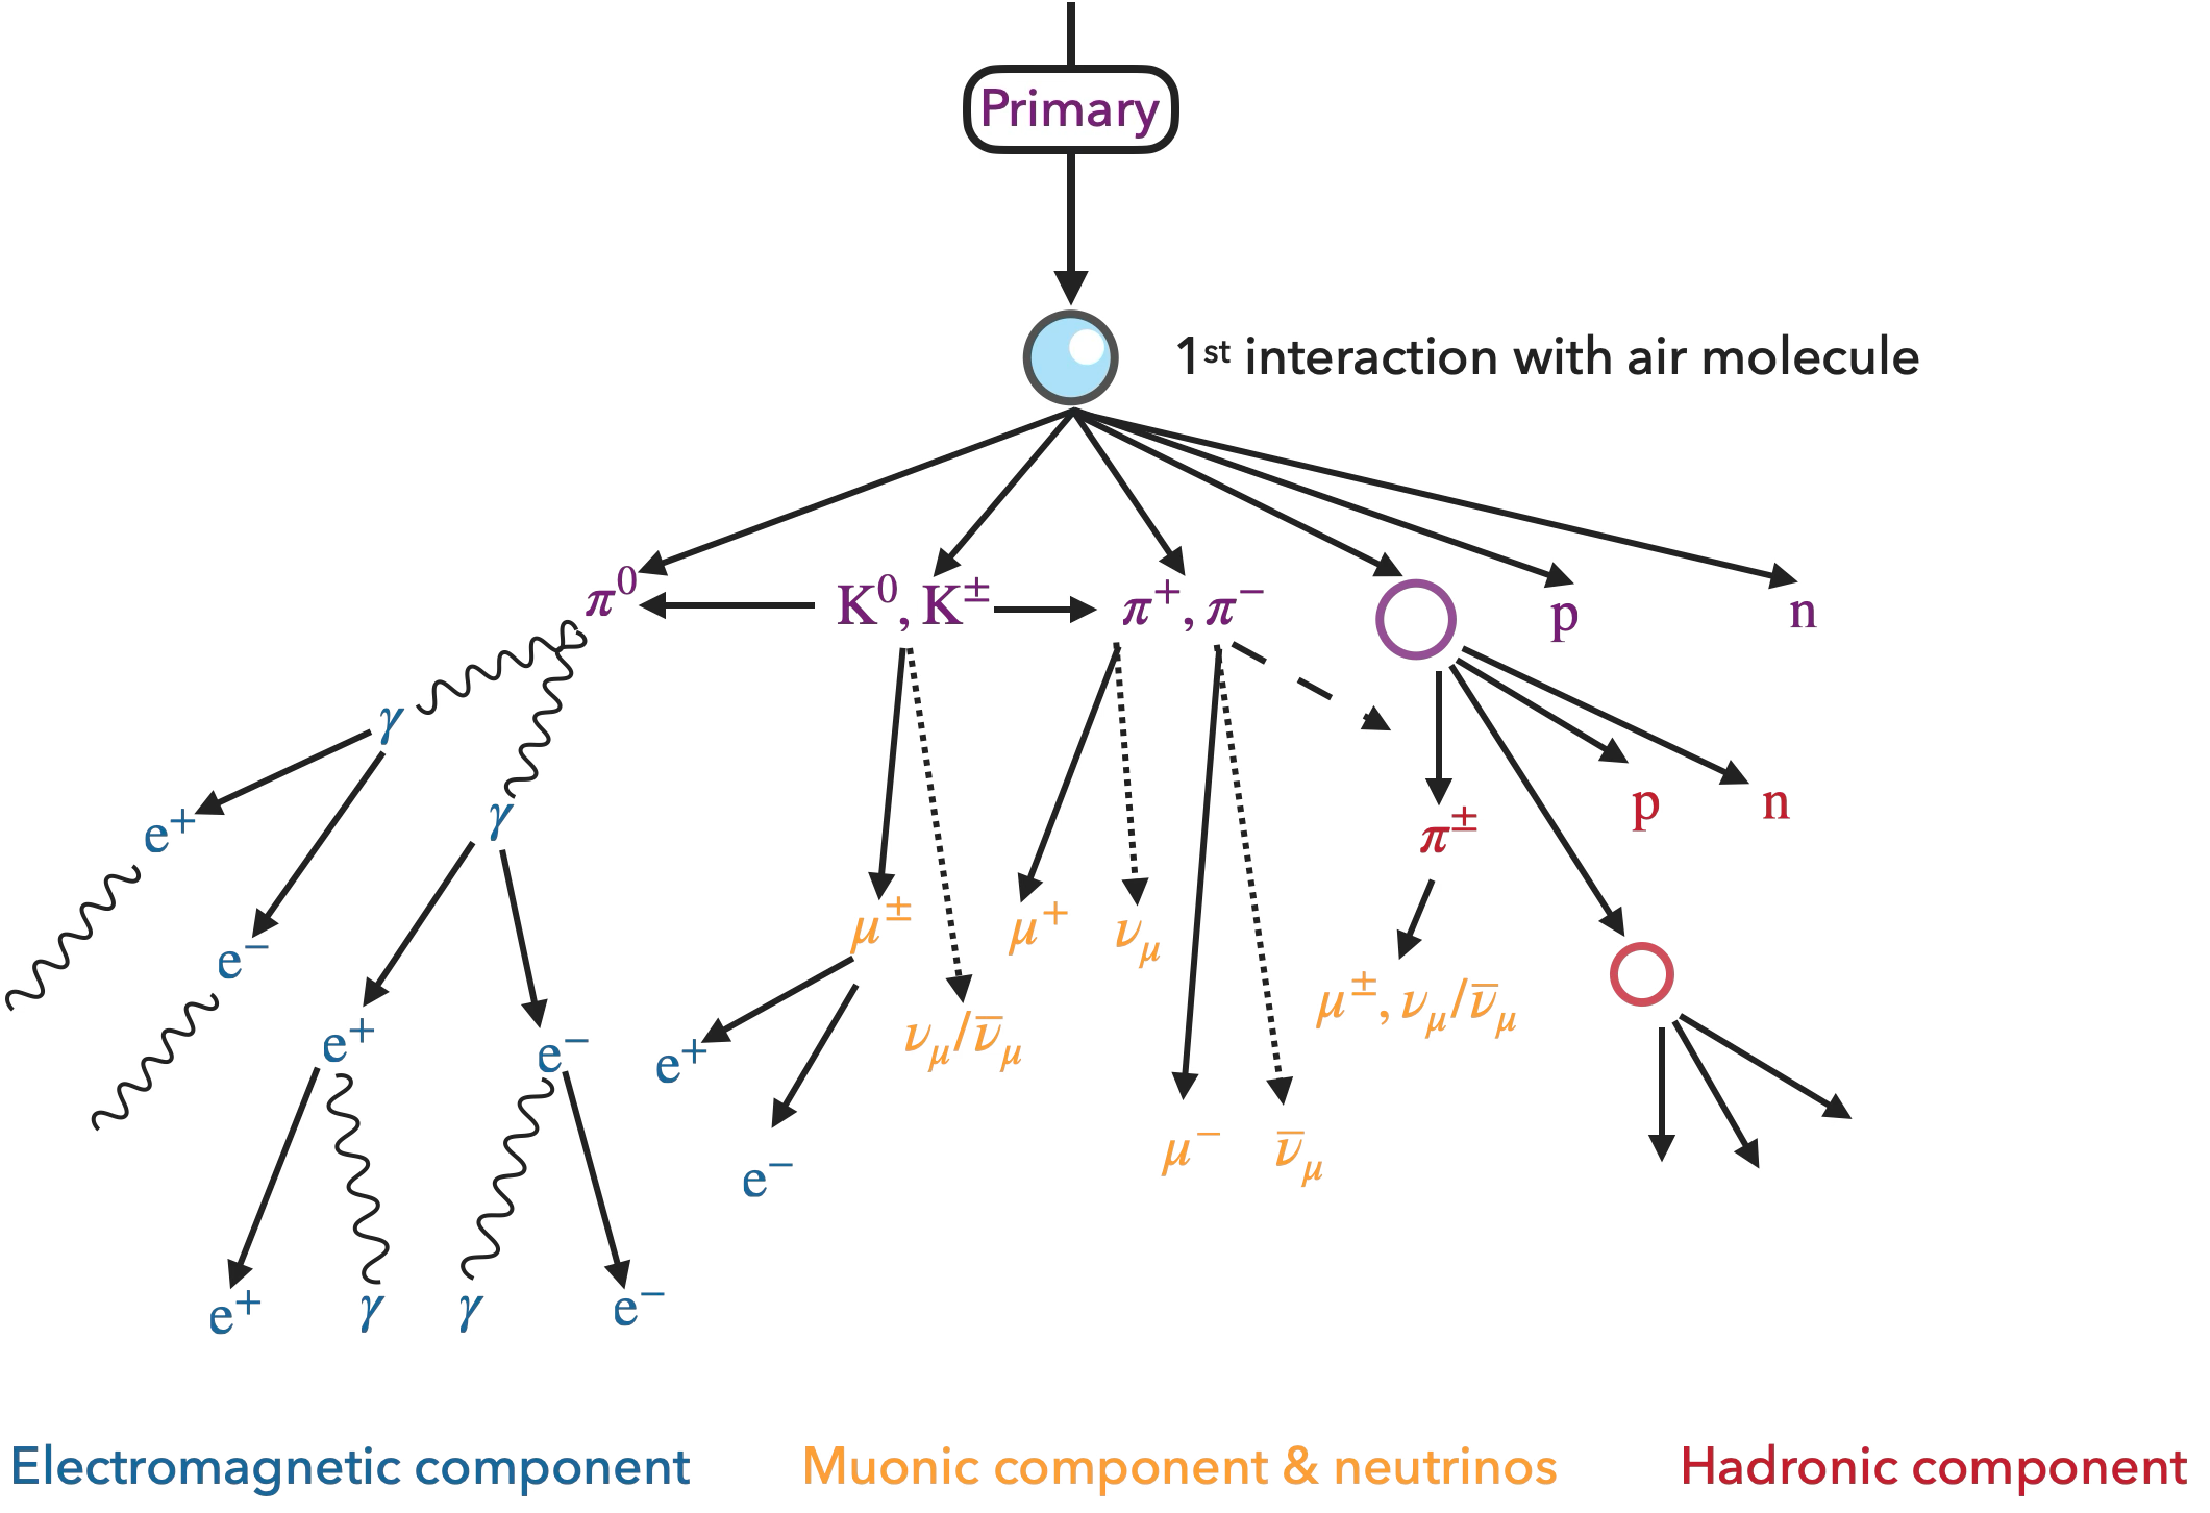
\includegraphics[width=14.5cm]{thesis_figures/EAS/EAS_reactions.pdf}
    \caption{Development of Extensive Air Shower. The figure shows the different components of an EAS and the reactions which lead to their formation.}
    \label{fig:EAS_components}
\end{figure}

\section{Development}
\label{sec:EAS_dev}

As the CR particle, which is predominantly a proton, collides with the nuclei of the atmosphere ($N_2, O_2 $,etc.) it produces pions and a few kaons. The neutral pions produced almost immediately decay to pairs of photons which in turn produce electrons via the process of pair-production. These electrons can then further produce photons via bremsstrahlung initiating a chain reaction which alternates between these two processes and forms the \textit{electromagnetic component} of the shower. The charged pions can survive for a while but eventually decay to muon and a corresponding anti neutrino. These muons can either survive till the shower reaches the ground and form the \textit{muonic component} or can also decay to electron thus contributing to the electromagnetic part. The neutrinos due to their low interaction cross-section mostly survive till they reach the ground and even further. Though not causing any problem for an EAS detector such neutrinos are the biggest background for a neutrino telescope. Kaons and charged pions due to their long lifetimes can also interact with the atmospheric nuclei producing additional pions which form the \textit{hadronic component} of the shower. The hadronic component can further contribute to both the electromagnetic and muonic component as more the shower propagates lesser the overall hadronic component becomes. A schematic of all the reactions with the different components is presented in Fig.~\ref{fig:EAS_components}.

To understand the cascade of particles a detailed modelling of each component is required. These models help extract the basic properties of the cascade. A simplified model describing the electromagnetic component called the Heitler's toy model, its hadronic extension, and a generalized cascade equation are all discussed below. The specific development of a neutrino induced EAS is also discussed.  
% \begin{figure}[t!]
%     \centering
%     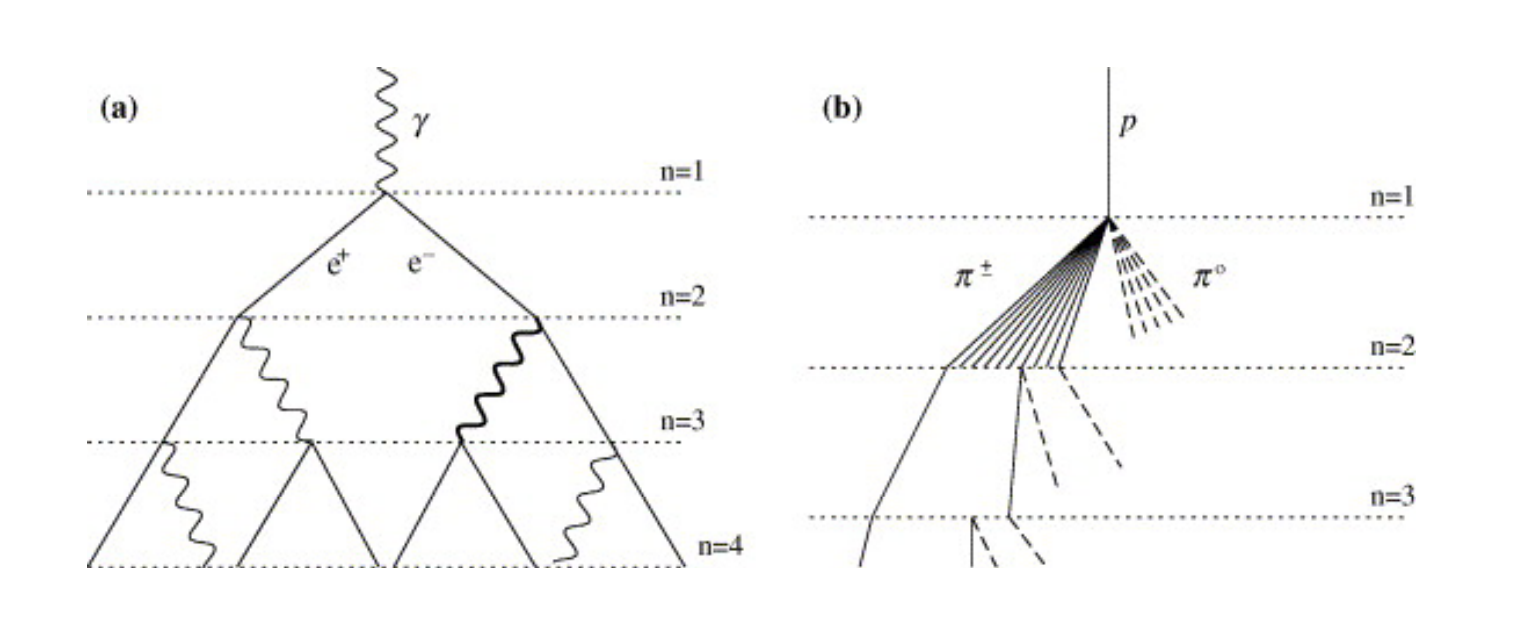
\includegraphics[width=14.5cm]{thesis_figures/EAS/Toy_mode_redo.png}
%     \caption{Representation of Heitler's model for (a) electromagnetic cascades and (b) hadronic cascades.} 
%     \label{fig:EAS_toy_model}
% \end{figure}

\begin{figure}[t!]
    \centering
    \subcaptionbox*{Electromagnetic cascades\label{sub:fig:toy_em}}{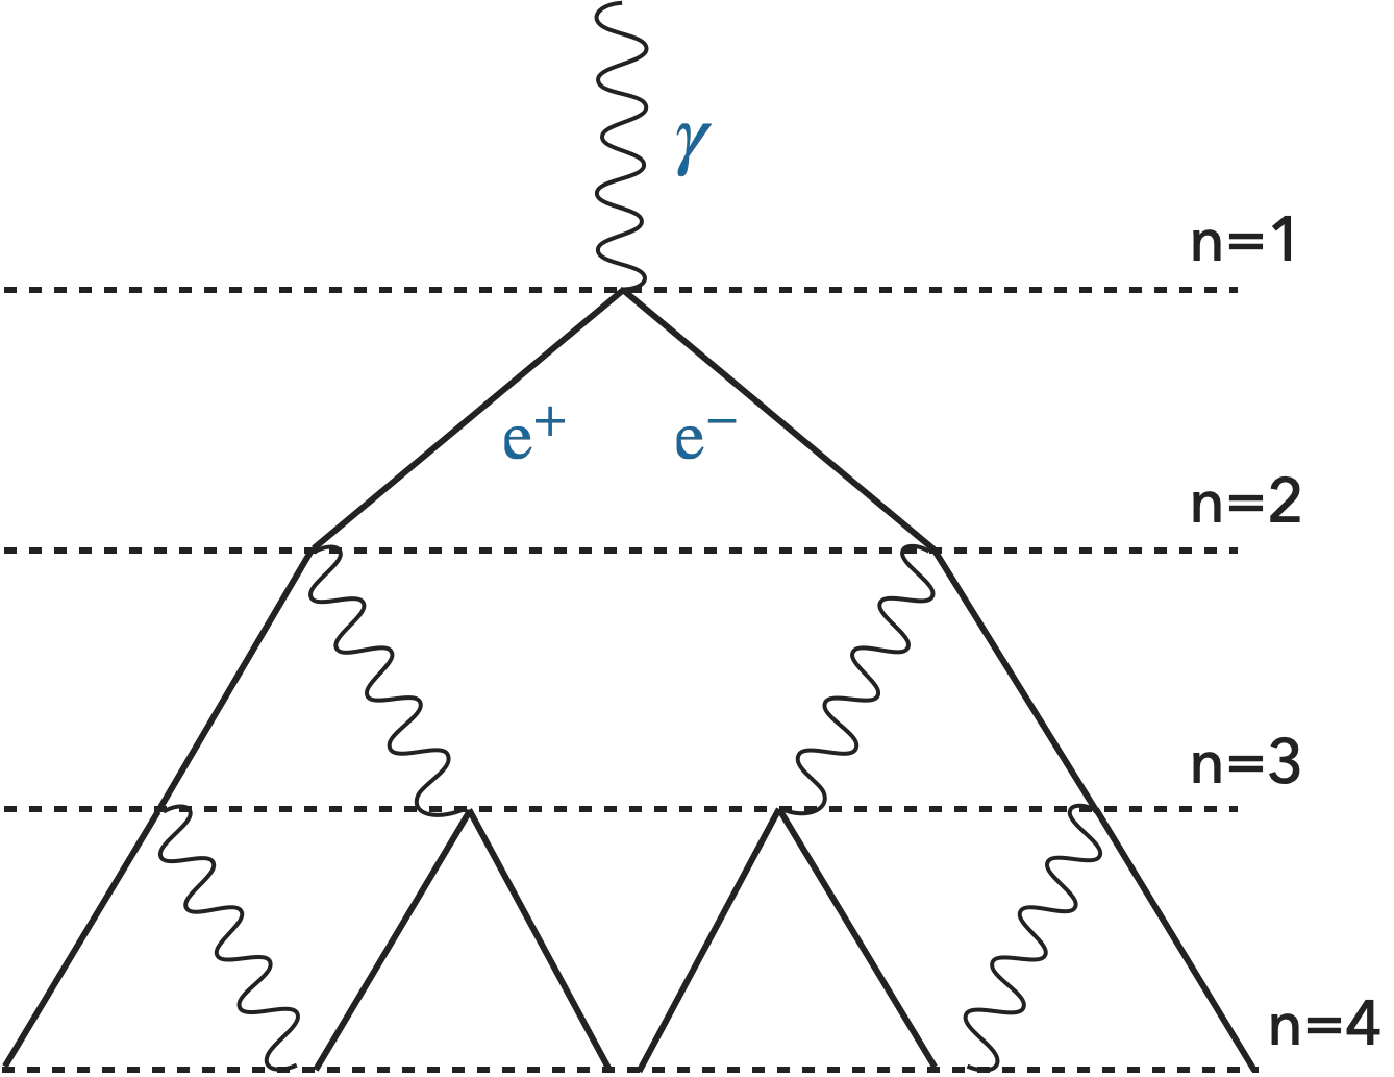
\includegraphics[width=.45\linewidth]{thesis_figures/EAS/Toy_model_em.pdf}}
    \hfill
    \subcaptionbox*{Hadronic cascades\label{sub:fig:toy_had}}{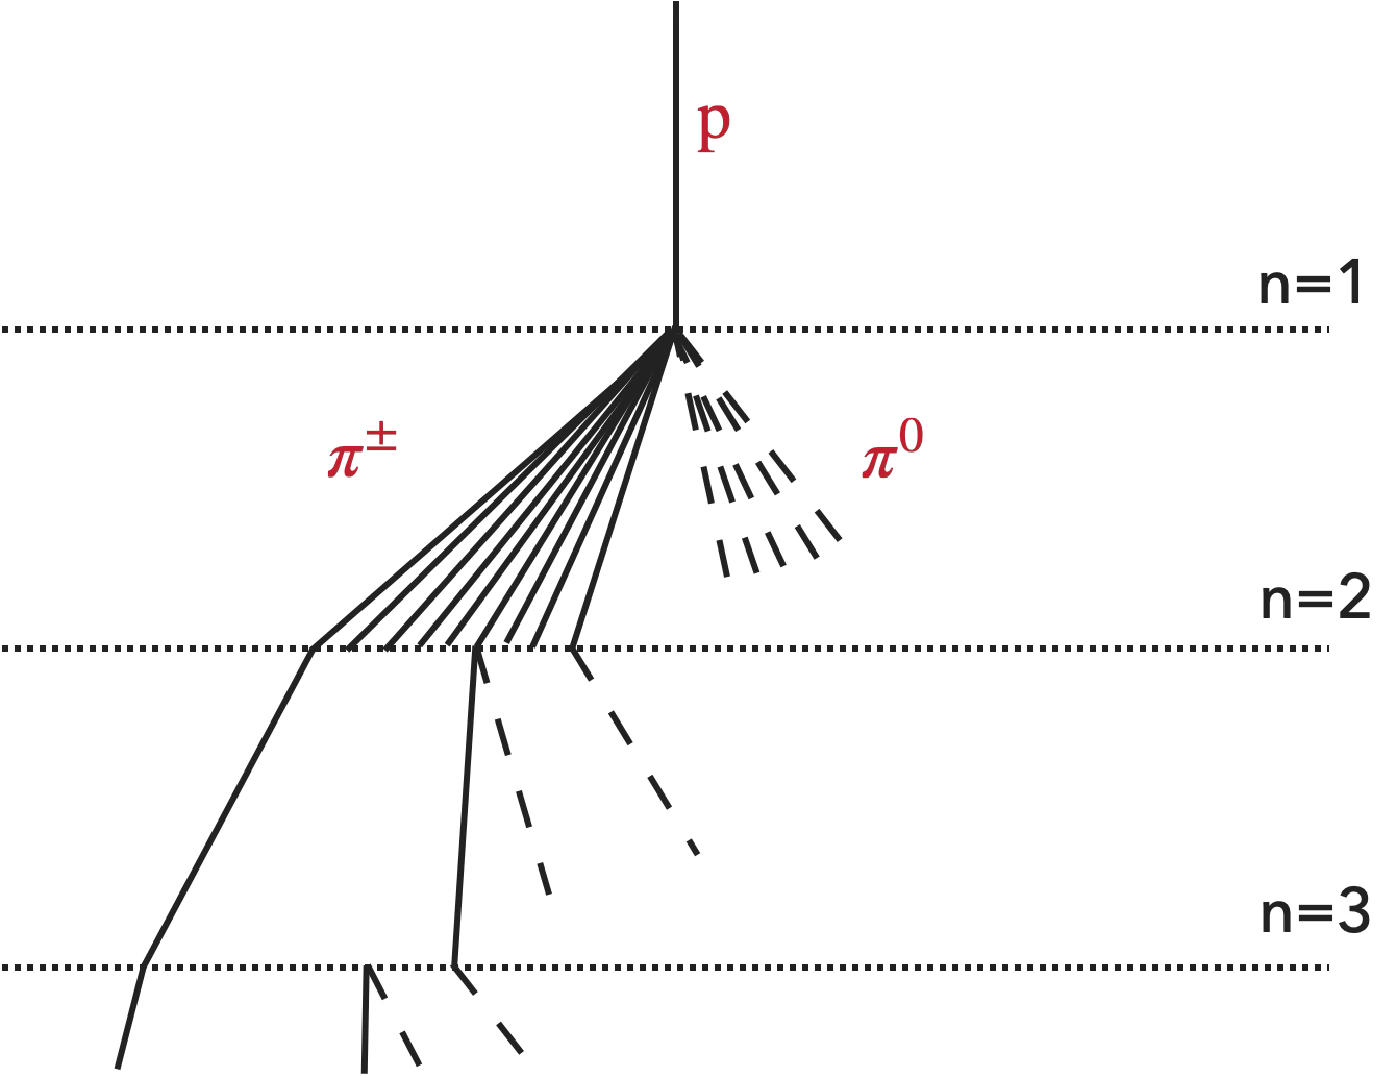
\includegraphics[width=.45\linewidth]{thesis_figures/EAS/Toy_model_had.pdf}}
    \caption{Representation of Heitler's model.}
    \label{fig:EAS_toy_model}
\end{figure}

\subsection{Heitler's Toy Model}
\label{sec:Dev_Heitler}

Proposed by Heitler in 1954~\cite{heitler1984quantum}, Heitler's Toy Model is a simplified perfect binary tree to understand and model an EAS development. The model characterises an EAS as a perfect binary tree. In such a scenario all particles produced in a shower equally share the primary energy available at the time of their creation. At each step, which has a fixed size related to the radiation length of the medium $\lambda$, the number of particles are supposed to be doubled, with each having the same energy. The energy losses which may occur due to collisions are completely ignored. The shower development or splitting process is supposed to continue until a critical point where the energy required to create more particles becomes the same as energy lost by particles in the medium. At the critical point, the shower has the maximum number of particles given by, $N_{\text{max}} = E_0/E_c$, which is the ratio of the original energy ($E_0$) to the critical energy ($E_c \sim 87$MeV). After this point the shower keeps getting absorbed in the atmosphere. The penetration depth at this point is called the shower maximum denoted by $X_{\text{max}}$. This can be calculated to be $X_{\text{max}} = X_0 + \lambda_r \ln(E_0/E_c)$ where $X_0$ is the first interaction point in the atmosphere. A visualisation of the shower development according to the Heitler's model is shown in Fig.~\ref{fig:EAS_toy_model}.

Such a simplified model works quite well for estimating the properties of the electromagnetic cascades although the $N_{\text{max}}$ estimations do not match perfectly. The reason for this is the difference in the energy loss values for electrons and photons. For hadronic cascades an extension to the model was made. Other important properties of the shower such as lateral and longitudinal spread, also require taking into account the emittance direction and losses due to collision which are not taken into account for a simplified model. These are discussed in sec.~\ref{sec:EAS_cha}. Even with its shortcomings the Heitler model gives a very good estimation for electromagnetic cascades and helps clearly categorise an air shower into three phases, the growth phase, the critical point phase and the tail phase. 

\subsection{Hadronic Extension}
\label{sec:Dev_Had}
The Heitler model was extended by Matthews~\cite{MATTHEWS2005387} to characterise the hadronic cascades in an EAS. In his approximation when a hadron with Energy, $E$ interacts with a nucleon the total particles produced have a two-third charged component ($\pi^\pm $) and a one-third neutral component ($\pi^0$) with the initial energy equally divided based on the number fraction. The neutral component decays quickly and contributes its share of energy to the electromagnetic component. The charged hadrons, provided they have not reached their critical energy in air ($\sim$20 GeV), interact again repeating the initial process. Muons are only produced when the charged hadrons acquire an energy below the critical energy. The energy transfer for each component after $n$ generations is given as $E_{\text{had}} = \biggl(\frac{2}{3}\biggr)^n E_0$ and $E_{\text{em}} = \big[1- \biggl(  \frac{2}{3}\biggr)^n\big] \, E_0$. Deeply penetrating air shower i.e a primary with high energy and a low enough cross-section in air, results in a lower number of muons produced, and observed at ground. This fact is important as based on the ratio of muons to electrons observed at ground, the type of the primary can be estimated. The number of muons ($N_{\mu}$) can be estimated in this model directly from charged hadrons when their energy falls below the critical energy. For $n$ generations one finds, $N_{\mu} = n_{\text{ch}}^n$ where $n_{\text{ch}}$ is the number of charged hadrons and $n$ can be written as $n = \frac{\ln(E_0/E_c)}{\ln(n_{\text{tot}})}$. Generalising by eliminating generations:

\begin{equation}
    N_{\mu} = \biggl(\frac{E_0}{E_c}\biggr)^{\alpha} , \, \alpha = \frac{\ln (n_{\text{ch}})}{\ln (n_{\text{tot}})}
\end{equation}

All the parameters in this model need to be estimated using detailed simulations~\cite{PhysRevD.66.033011}. $\alpha$ has been estimated to be in the range 0.82...0.9. Other factors such as production of particles which do not decay such as baryon-anti-baryon pairs~\cite{ Pierog:2006qv} can also affect the calculated values in this model. Other than the shower maximum and number of muons, the change of the depth of the shower maximum per decade in energy also called the elongation rate is given by $D_{10} = \frac{\left\langle X_{\text{max}}\right\rangle }{d\log_{10}E_0} = 2.3\lambda_r$. The elongation rate of electromagnetic showers in air is about $\approx 85\,\text{g cm}^{-2}$. The elongation rate theorem~\cite{Linsley_1977} states that the upper limit to the elongation rate for hadronic showers is also $D_{10}^{\text{em}}$ in the presence of Feynman scaling.

The first interaction with the nucleon was presented in a simplified way by Matthews as the superposition model. In this model a nucleus with mass A is assumed to be a superposition of $A$ independent nucleons, each with energy $E_h = E_0/A$. With such an assumption one can reach the following conclusions:

\begin{description}
    \item $N_{\text{em, max}}^A(E_0) = A N_{\text{em, max}}^h(E_h/E_c) \approx N_{\text{em, max}}(E_0) $ i.e. the fraction of energy transferred to the electromagnetic component at shower maximum, has only an indirect dependence on the primary mass via the dependence on primary energy.
    \item $X_{\text{max}}^A(E_0) = X_{\text{max}}(E_0/A)$. This shows how the shower maximum has an inverse dependence on the mass of the primary i.e a shower initiated by heavier nuclei will develop higher in the atmosphere compared to one initiated by lighter nuclei.
    \item $N_{\mu}^A(E_0) =  A \biggl(\frac{E_0/A}{E_{c}}\biggr)^{\alpha} = A^{1-\alpha} \biggl(\frac{E_0}{E_c}\biggr)^{\alpha}$. This shows that heavier primaries will produce a larger number of muons compared to lighter primaries. For e.g. Iron showers on average contain 40\% more muons than proton showers~\cite{Fowler_2001}.
    \item $D_{10} = D_{10}^{\text{had}} \Biggl(1- \frac{d\left\langle ln A\right\rangle}{d\log_{10} E}\Biggr)$ Since Feynman scaling is known to be violated for higher energies, the hadronic elongation rate is always less than the electromagnetic rate. Thus, an increase in elongation rate towards 85 g cm$^{-2}$ is a direct indication of change of the mass composition. 
\end{description}
Simulations have shown that the superposition model gives a more realistic description of many features of the shower~\cite{Wibig_2022}. However, it is still not a perfect description especially for heavier nuclei. Studies with photographic emulsion techniques have tried to create a better picture of the fragmentation of heavier nuclei~\cite{LI2013503}. This field is continuously evolving with better models and theoretical predictions being worked on based on the continually increasing database of observations. 

Although these models help understand the principle, a full Monte Carlo simulation and a generalised analytical solution of the cascade equations is needed to fully recreate the EAS. Even after huge amount of efforts made a few discrepancies such as the muon puzzle which is the mismatch in the number of muons predicted by the simulations in comparison to the measurements remain~\cite{Albrecht_2022_muon_puzzle}.  

\subsection{LPM effect}
\label{subsec:LPM}
Another process that can directly impact the development of highly energy electromagnetic showers is the Landau-Pomeranchuk-Migdal effect~\cite{Landau:1953um,PhysRev.103.1811}. The LPM effect is the reduction of the bremsstrahlung and the pair-production cross-section at high energies or densities. All the above models work under the assumption that the energy range is low enough for the LPM effect to not be applicable. If the medium is dense enough or at high energies the LPM effect also becomes important to fully estimate the development of an air shower. The implications of the LPM effect for air showers implemented in simulations can be found in~\cite{sandrock2023validationelectromagneticshowerscorsika}. 

\subsection{Neutrino induced EAS}
\label{sec:Dev_Nu}
The development of a neutrino induced shower in comparison to a CR shower is important in the context of this study. Understanding the differences helps to identify the unique signature at a CR observatory like the Pierre Auger. The differences in the shower development can also help increase the sensitivity of a neutrino observatory like the IceCube. Unlike a cosmic ray particle a neutrino can interact at any depth. This is due to the low neutrino cross-section at $10^{18}\,$eV $\approx 10^{-33} \mathrm{cm^2}$  in comparison, for e.g. the proton-nucleon cross-section which is $\approx 10^{-27} \mathrm{cm^2}$. Thus, neutrino-induced showers require significantly higher neutrino energies to produce interactions with observable effects. The main channel via which an ultra-high energy neutrino can interact is either a CC or NC interaction as mentioned in the last chapter. Neutrino-induced showers involve fewer particles in the initial interaction which translates to difference in the shower development in comparison to CR induced air showers. The development of the shower and the unique signature depend on the flavor of the neutrino as shown in fig~\ref{fig:NU_EAS_channels}.
% \begin{figure}[t!]
%     \centering
%     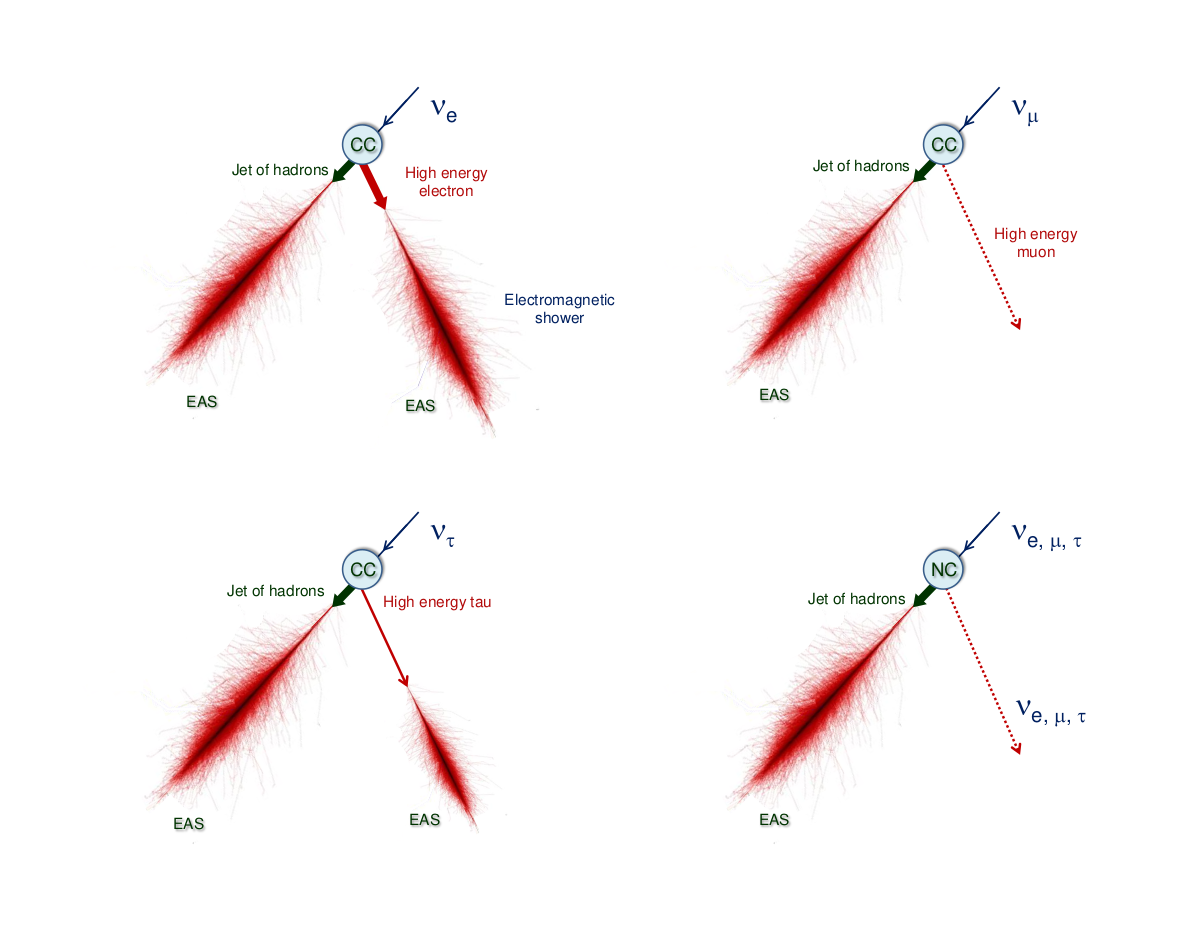
\includegraphics[width=14.5cm]{thesis_figures/EAS/Nu_EAS_channels.png}
%     \caption{Sketch of different possible interactions of UHE neutrinos in the atmosphere. } 
%     \label{fig:NU_EAS_channels}
% \end{figure}
\begin{figure}[t!]
    \centering
    \subcaptionbox*{ \label{sub:fig:e_CC}}{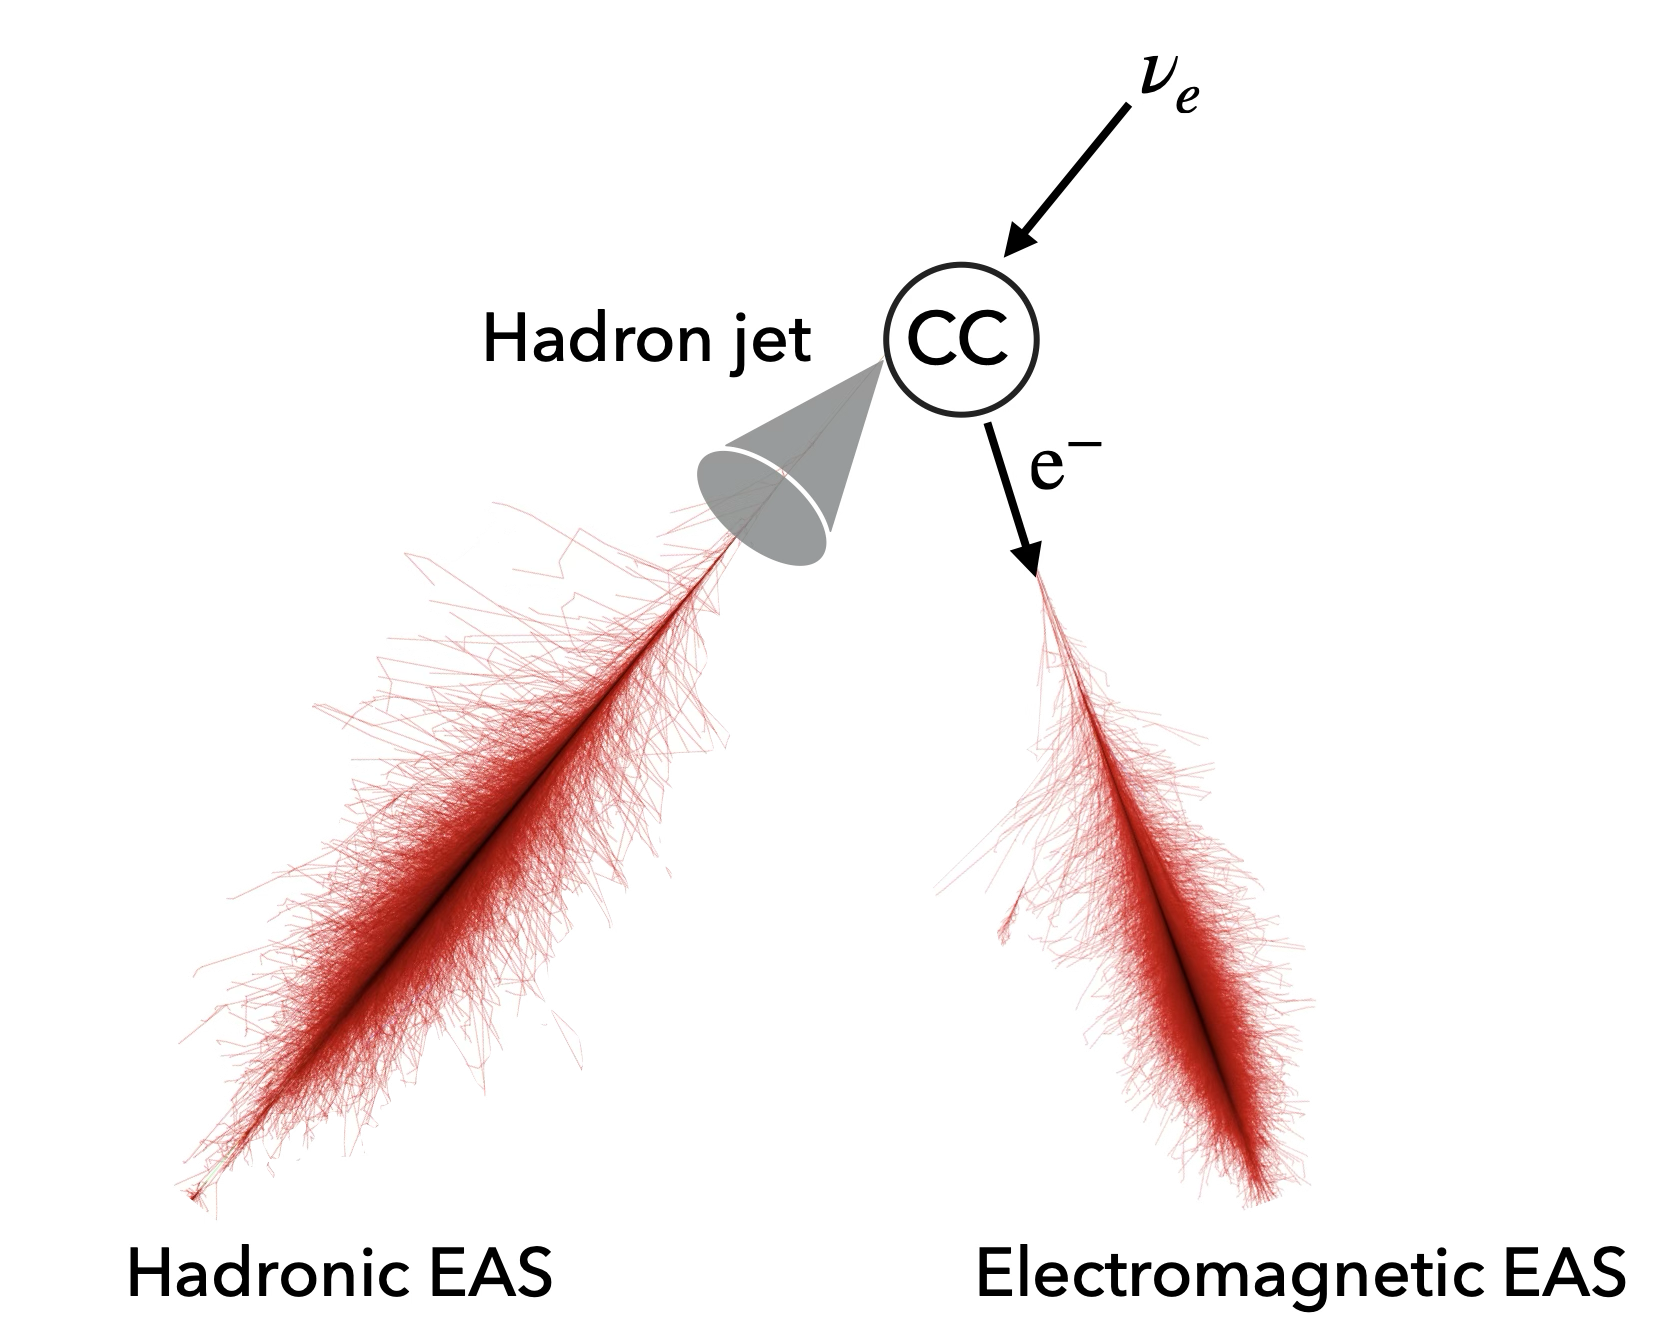
\includegraphics[width=.45\linewidth]{thesis_figures/EAS/e_CC.png}}
    \hfill
    \subcaptionbox*{ \label{sub:fig:mu_CC}}{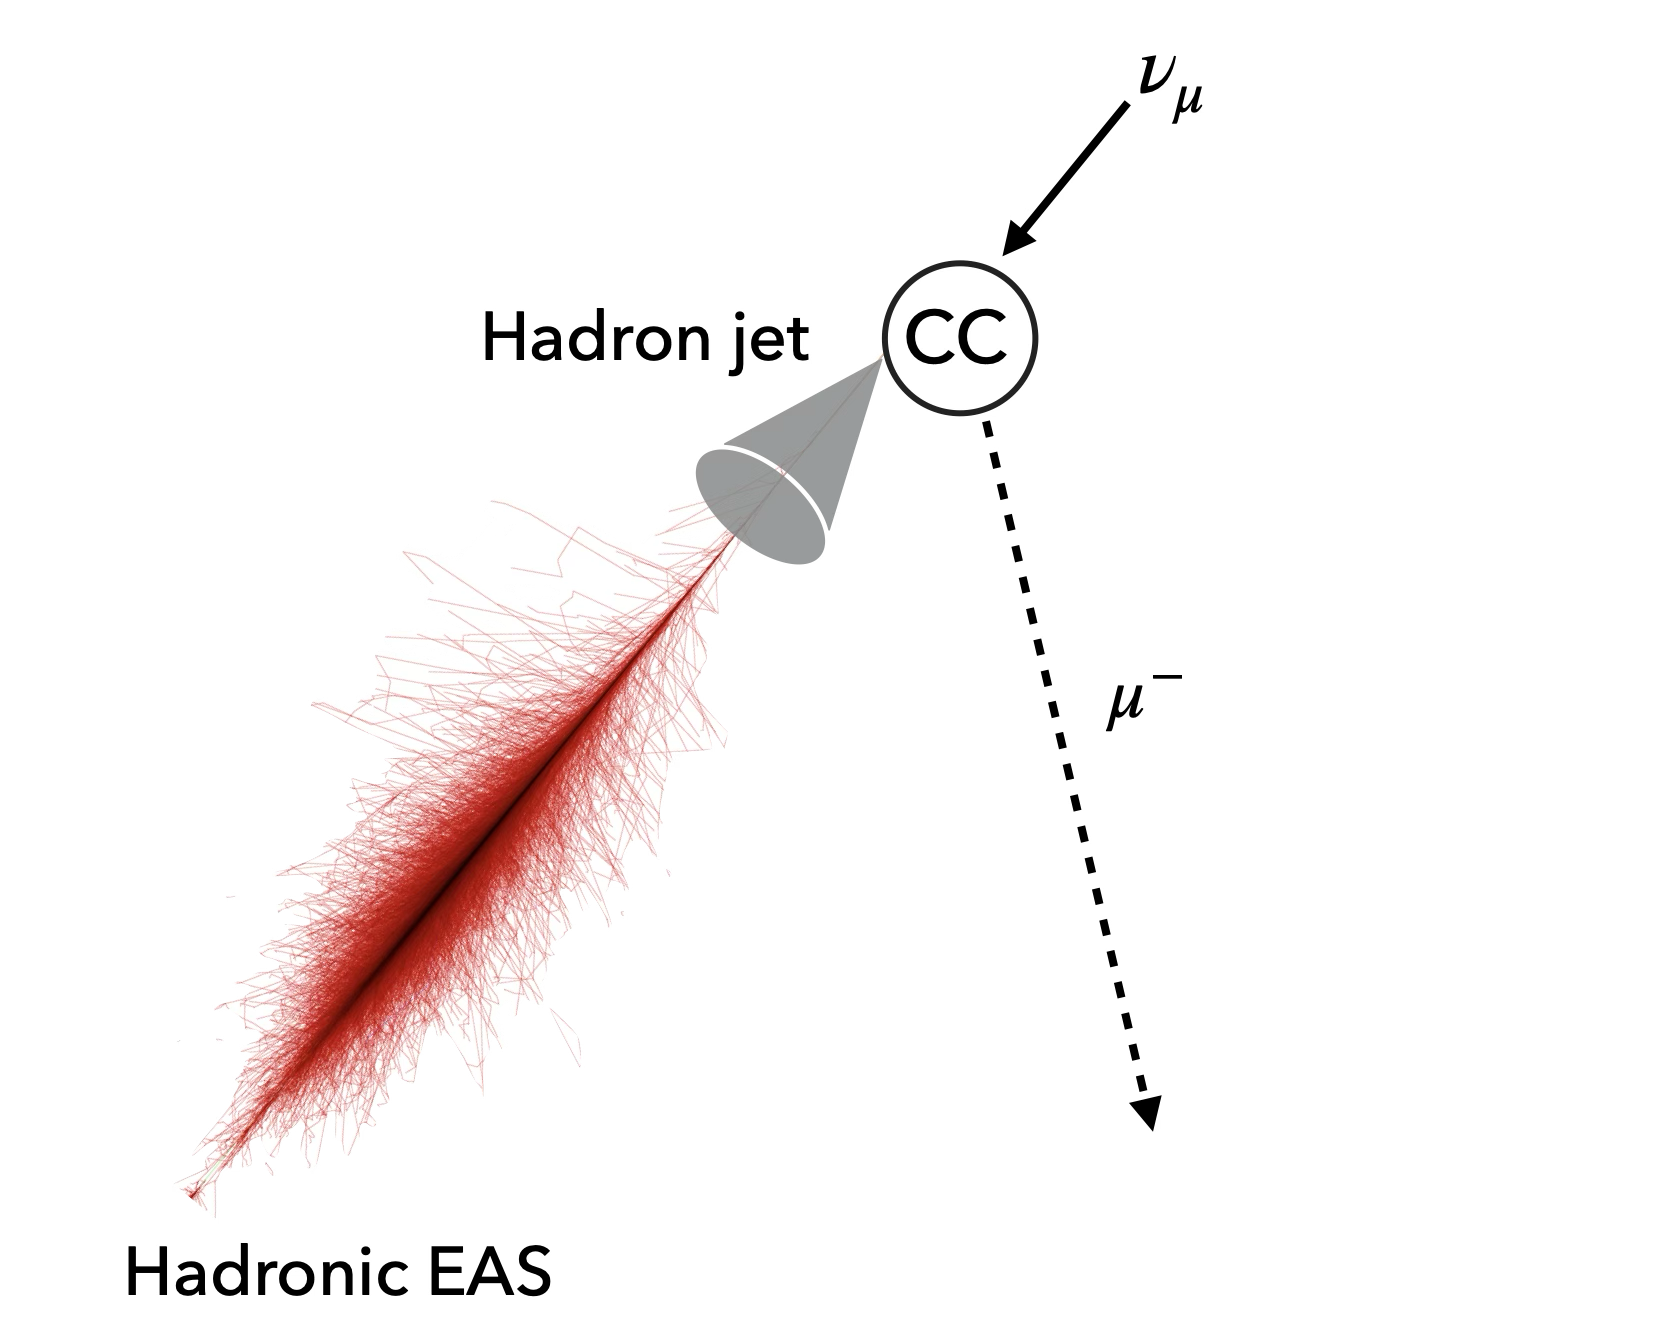
\includegraphics[width=.45\linewidth]{thesis_figures/EAS/mu_CC.png}}
    \hfill
    \subcaptionbox*{ \label{sub:fig:tau_CC}}{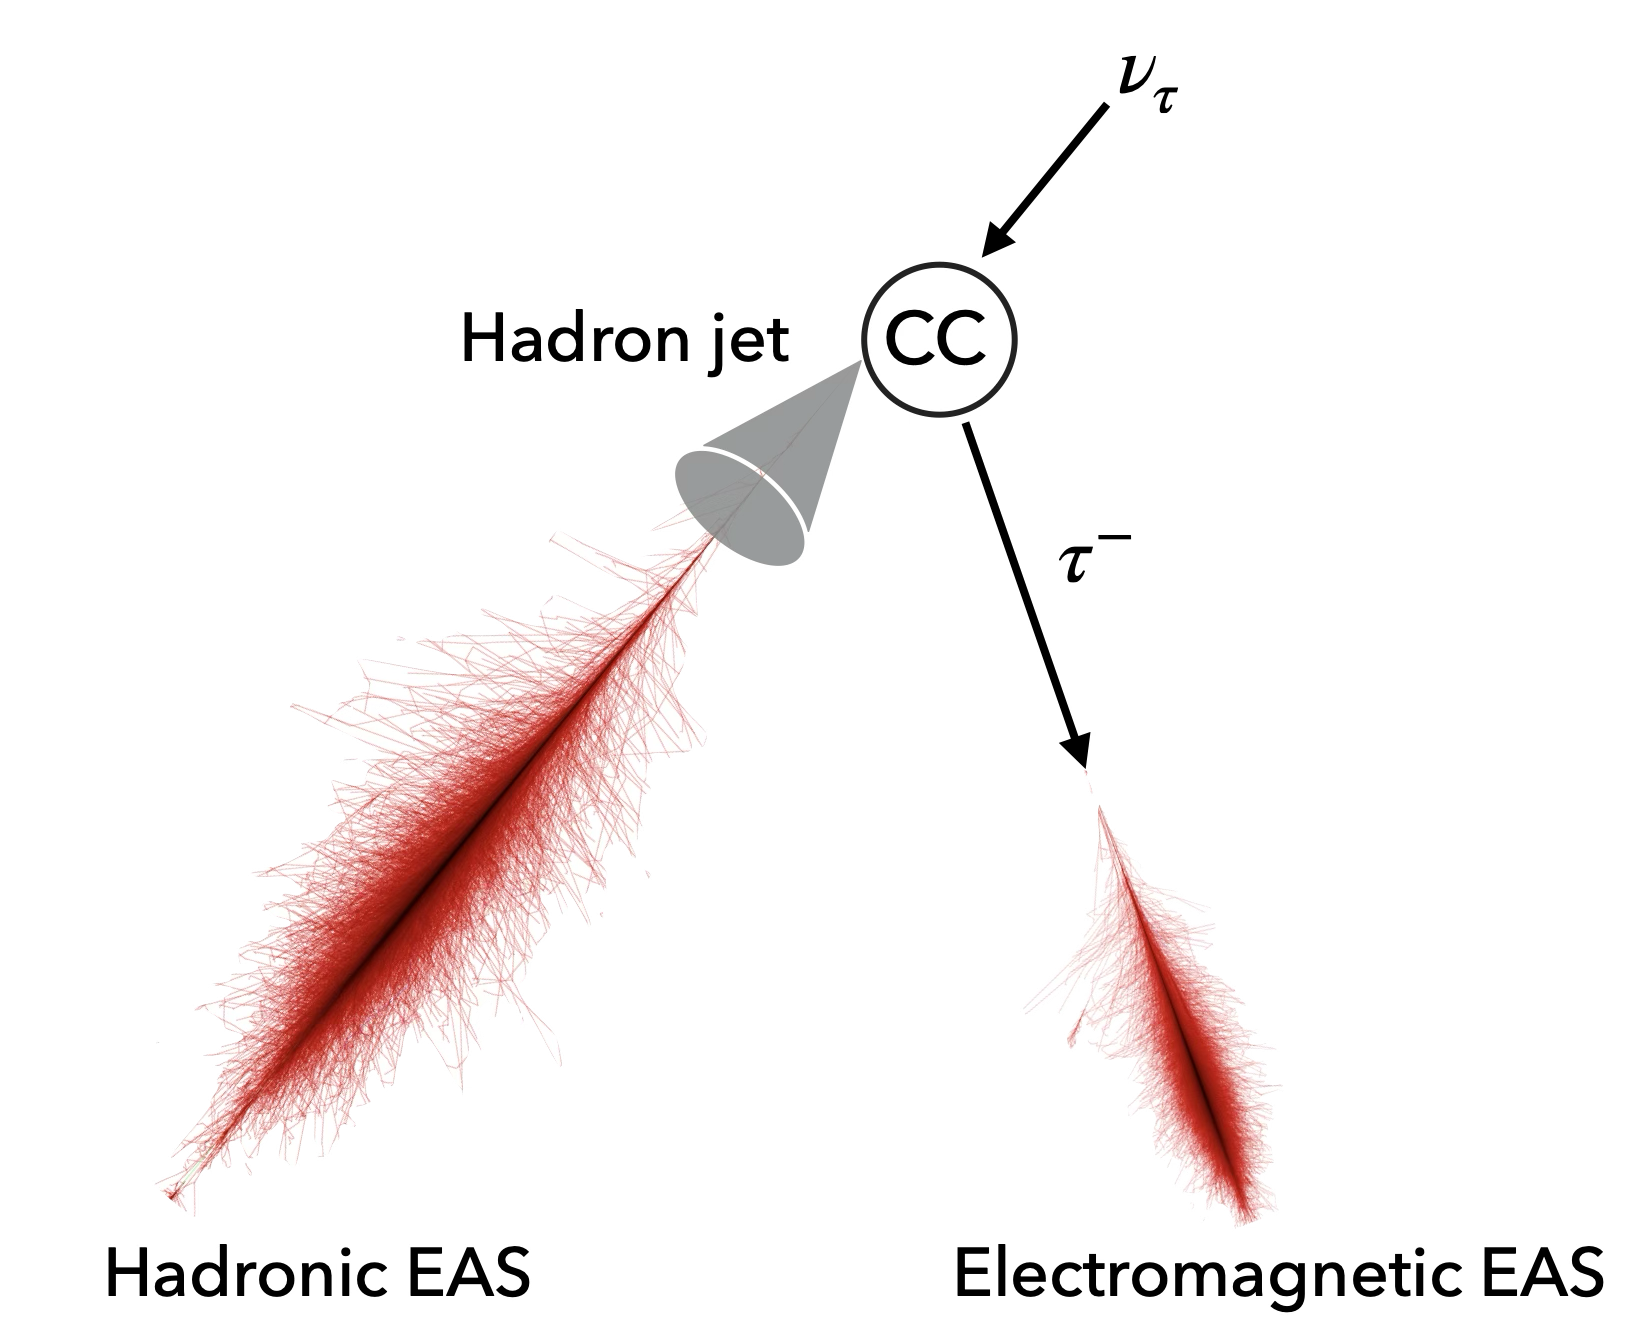
\includegraphics[width=.45\linewidth]{thesis_figures/EAS/tau_CC.png}}
    \hfill
    \subcaptionbox*{ \label{sub:fig:nu_NC}}{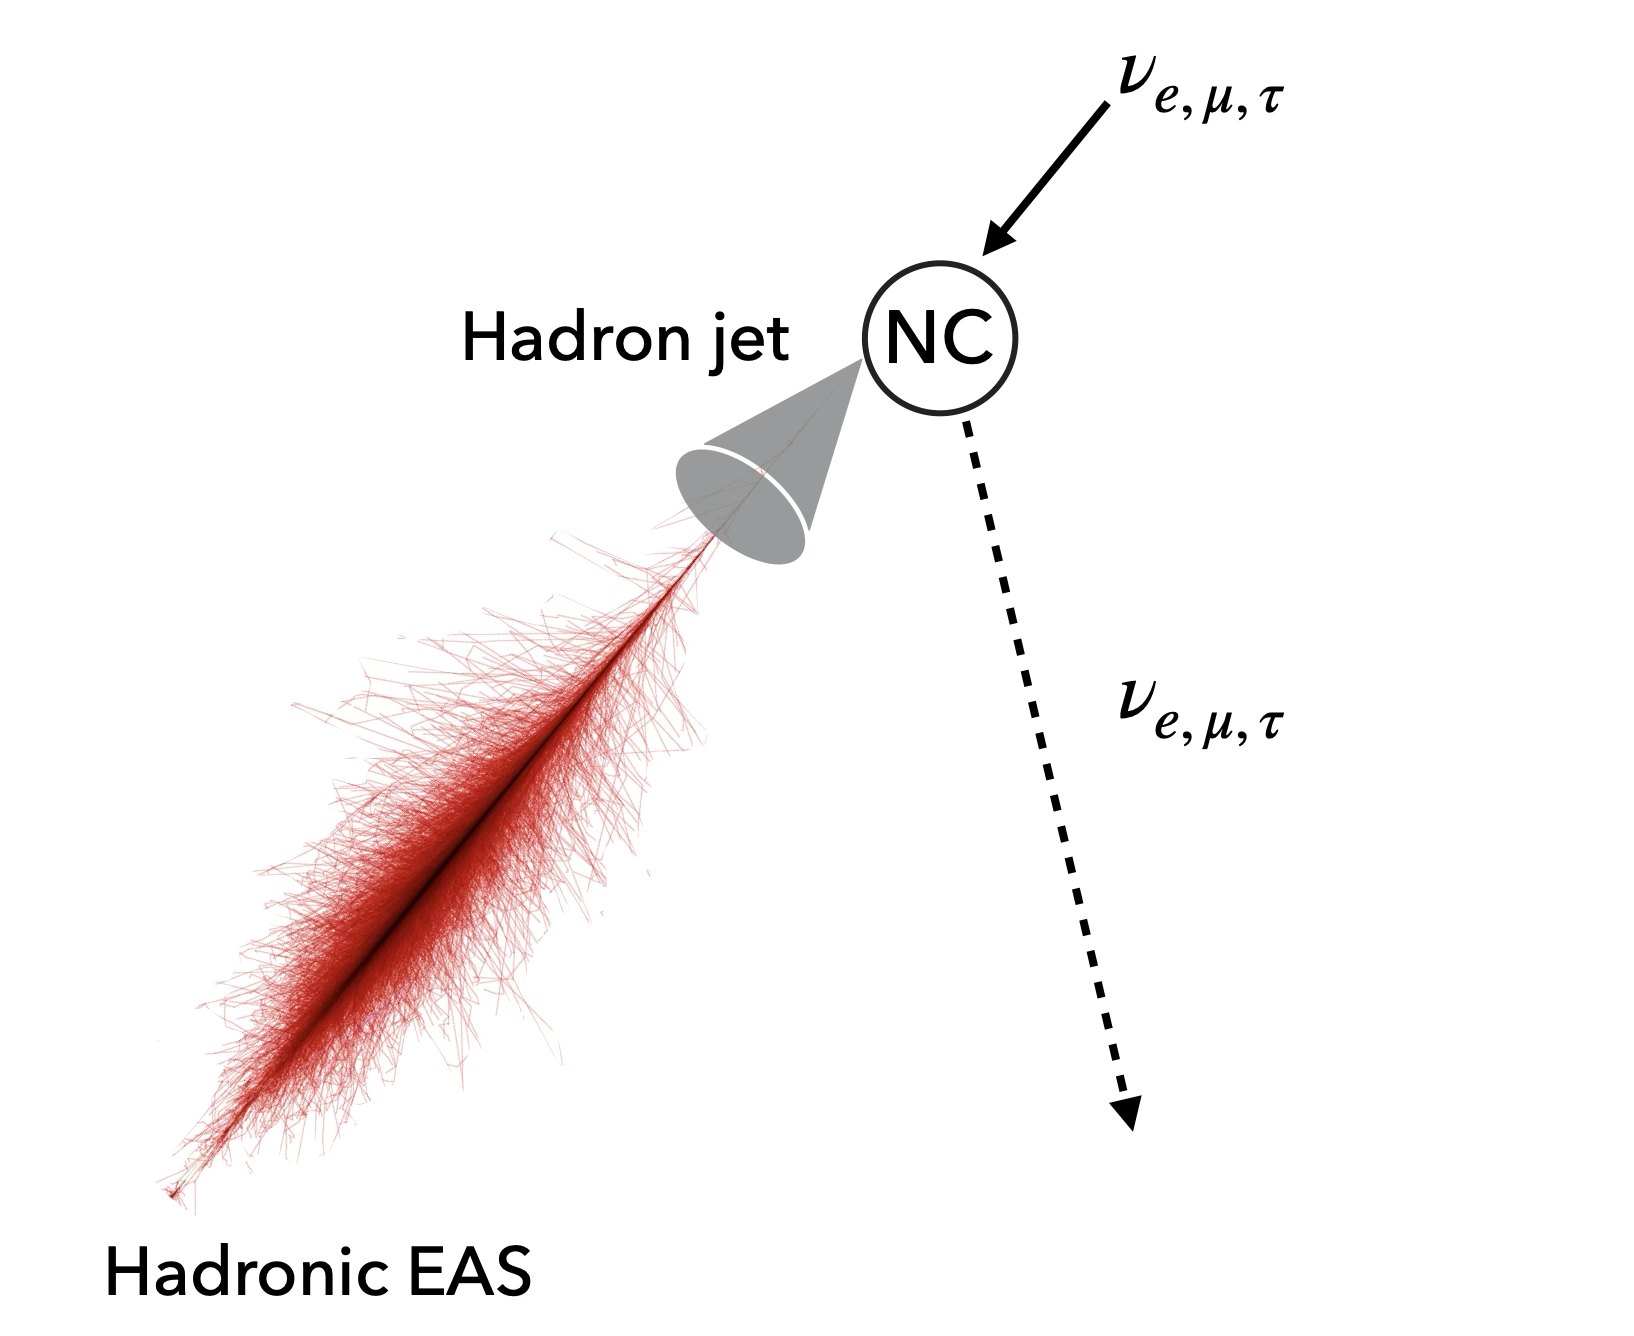
\includegraphics[width=.45\linewidth]{thesis_figures/EAS/nu_NC.png}}
    \caption{Sketch of different possible interactions of UHE neutrinos in the atmosphere.}
    \label{fig:NU_EAS_channels}
\end{figure}

An electron neutrino, $\nu_e$, interacting via CC interaction produces an initial hadronic cascade which has fewer particles in comparison to a hadron-initiated shower from the CRs. The high energy electron/positron produced in the same initial interaction also produces an electromagnetic shower. At high energies the two showers are overlapped and the fraction of energy carried by the electron/positron governs the ratio of the electromagnetic to hadronic component for the shower.

A muon neutrino, $\nu_{\mu}$, also produces an initial hadron cascade but in contrast to the electron neutrino interaction the resulting muon has a very low probability to decay and mostly passes through the detector undetected. The energy carried by the muon which is usually a large fraction is invisible and only the hadronic cascade can be detected.

Tau neutrinos, $\nu_{\tau}$, have a unique and particularly interesting signature among neutrino showers. The initial interaction remains the same with the production of a hadronic cascade, but the resulting tau lepton has a decay length $\approx$ 10 km. This means that depending on the atmospheric depth the tau encounters on its way to the ground, it can either decay and potentially produce an electromagnetic cascade much later than the initial hadronic cascade or not decay at all. The asynchronous cascade signature is also known as "double-bang" effect and can occur both in air or a specific medium. Tau neutrinos can also be a source of upward-going air showers which can also be detected at an EAS detector. In this case the tau neutrinos can interact in the Earth's crust or in some natural obstruction like mountains around the detector leading to production of a hadronic cascade which gets absorbed and a tau lepton which can escape and produce an electromagnetic cascade in air that can be detected. The process is unique to tau neutrinos for an EAS detector since for a $\nu_e$ both the hadronic cascade and the electron is absorbed by the obstacle whereas for the muon neutrino the resulting muon is almost impossible to detect.  

All three neutrino flavors can also undergo NC interactions. These also result in an initial hadronic cascade and a neutrino which usually does not interact and escapes being detected especially for an EAS detector. Thus, the signature is indistinguishable in comparison to a muon neutrino CC interaction. The probability of NC interaction is also lower than a CC interaction which also affects the overall number of EASs induced due to this channel.

\section{Characteristics}
\label{sec:EAS_cha}
Apart from the shower maximum and the number of muons at ground other observables are also required to fully characterise the shower and estimate the important quantities such as the mass, energy and the arrival direction of the incoming primary CR or UHE$\nu$. Fig.~\ref{fig:EAS_schematic} gives an overall picture of the evolution of an EAS. The amount of atmosphere penetrated is measured in units of slant depth X, with a unit of $\mathrm{g/cm^2}$. The first interaction depth, $X_0$, is the slant depth until the first interaction of the primary particle with the nucleon. The shower begins from this point on and the vector along which the shower develops from the first interaction point is called the \textit{shower axis}. The development continues till the shower reaches a maximum which was defined earlier and is denoted by $X_{\text{max}}$. After this point the shower depopulates which is caused by particle energy loss due to absorption or decay. The \textit{longitudinal development profile} plotted in Fig.~\ref{fig:EAS_schematic} gives a relation between the number of shower particle in dependence to the atmospheric depth. This relation is also called the Gaisser-Hillas function~\cite{1977ICRC....8..353G} parametrised as follows.

\begin{equation}
    N(X) =  N_{\text{max}} \biggl(\frac{X- X_0}{X_{\text{max}} -  X_0}\biggr)^{\frac{X_{\text{max}}-X_0}{\lambda}} \exp \biggl(\frac{X_{\text{max}}-X_0}{\lambda}\biggr)
\end{equation}

\begin{figure}[t!]
    \centering
    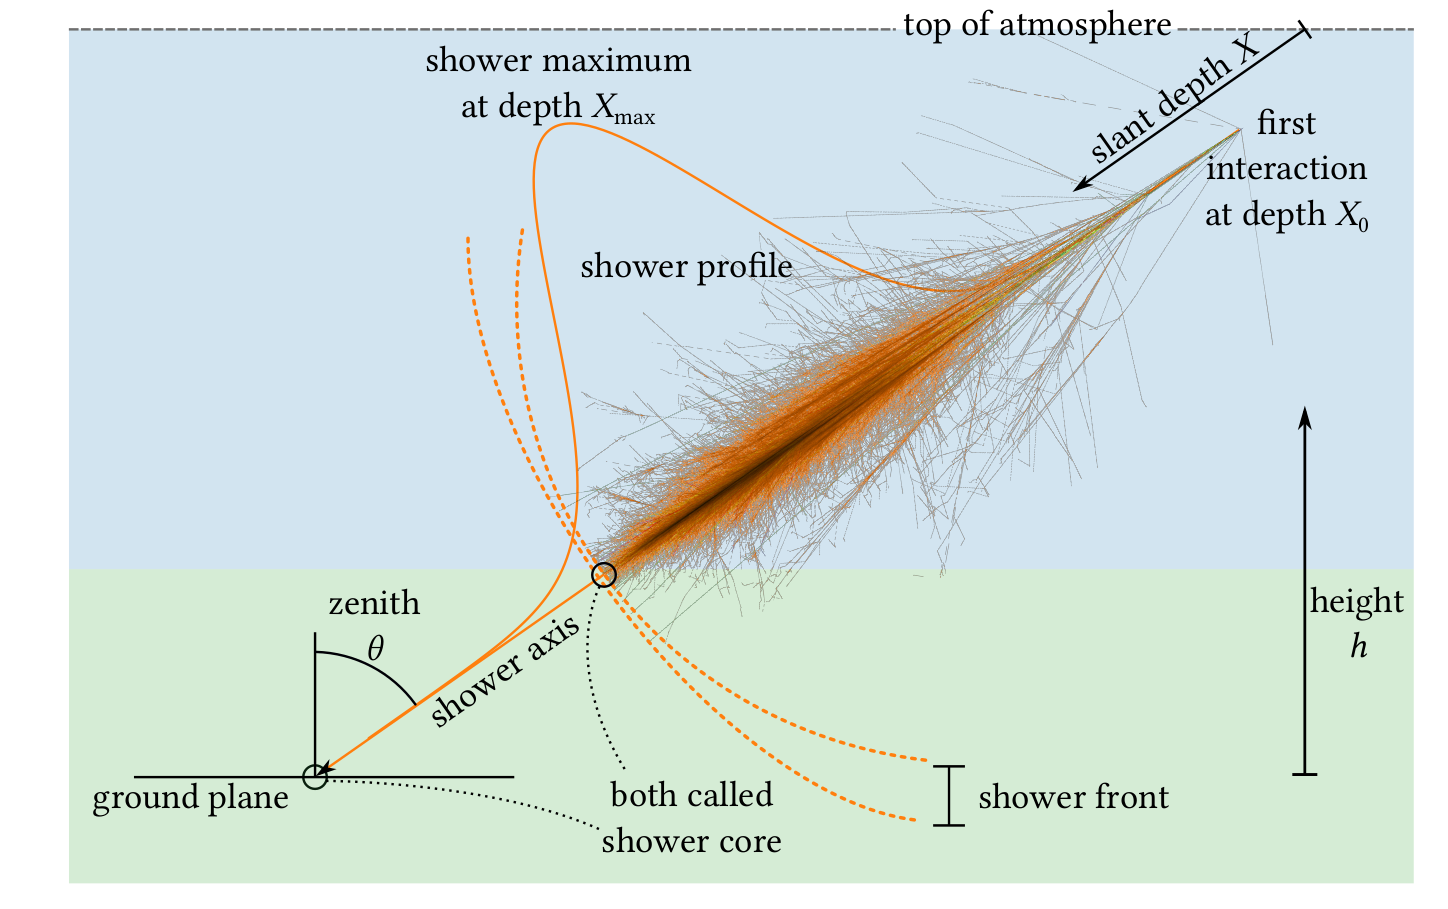
\includegraphics[width=14.5cm]{thesis_figures/EAS/EAS_schematic.png}
    \caption{Schematic of the development of an EAS in the atmosphere. Taken from~\cite{thesis:mayotte2021}.} 
    \label{fig:EAS_schematic}
\end{figure}

$X_0$ and $\lambda$ can be estimated by fitting the profile based on the above function and depend on the composition and energy of the primary. $N_{\text{max}}$ is the number of particles observed at $X_{\text{max}}$. The integral of the longitudinal development profile gives an estimate of the total calorimetric energy deposited by the shower. 
The point where the shower axis vector intersects the ground is called the \textit{shower core}. The shower axis is thus defined by the zenith angle $\theta$, azimuth angle $\phi$ and the shower core position. If one looks at the shower head on, the large thin disc like appearance consisting of highly energetic particles is called the \textit{shower front}. The shape is due to the path length differences between the shower particles travelling away from the shower axis to the one travelling in the direction of the shower axis. The disc is thus thinner near the shower core and widens away from it. As the shower front intersects the ground, the density and the timing of the particles detected at the detector form what is called the \textit{shower footprint}. It is the primary observable used by a ground level EAS detector to measure and characterise the shower. The arrival time of the particles in the footprint can help determine the shower geometry whereas the density can be used to reconstruct the energy of the primary. The density is estimated as a function of the radial distance from the shower core on the ground, by the \textit{lateral distribution function} (LDF). The modern LDF function is an extension on the parameterisation given by Greisen~\cite{annurev:/content/journals/10.1146/annurev.ns.10.120160.000431} and by Kamata and Nishimura~\cite{10.1143/PTPS.6.93} and is described as:
\begin{equation}
    \label{eq:Lateral_dist_func}
    \rho_e(r) = \frac{N_e}{2 \pi R_M^2} C(s) \biggl(\frac{r}{R_M}\biggr)^{(s-2)}\biggl(\frac{r}{R_M}+1\biggr)^{(s-4.5)}
\end{equation}

with shower ages $s$ and the Moliere radius $R_M = 0.0265 \,X_0(Z + 1.2)$.

Another important characteristic of an EAS are its universality features first pointed out by Hillas for electromagnetic showers~\cite{A_M_Hillas_1982}. In this formulation the average development of an air shower is universal around the shower maximum. An individual shower can be defined by the shower age given as:
\begin{equation}
    s = \frac{3}{1+2 X_{max}/X}
\end{equation}
This parameter is a result of the nature of the development of the cascade process which hides the initial primary dependent fluctuations~\cite{Fedosimova:2017vxz}. Simulations have used such a universal feature to fit shower profiles reasonably well independent of the primary mass and energy~\cite{Bridgeman:2017MD}. Air shower universality only holds for air showers induced by gamma rays, electrons, or positrons and breaks down for a hadronic cascade. It can still be used if each individual component of the shower can be disentangled. Although, not applicable for this study,universality is an important characteristic of the shower and has been used in various CR~\cite{cazon2024protonairinteractionsultrahighenergies} studies such as to estimation of the proton-air cross-section~\cite{Ulrich_2009} and other CR studies.

\section{Detection}
\label{sec:EAS_det}
At high energies, due to the low flux, EAS offer the best way to detect CRs. Ground based detectors can be spread over large areas offering a cost-effective way to study UHECRs. The particles arriving at ground can also be directly detected. Furthermore, the shower can be seen through different emissions such as the Cherenkov, fluorescence and radio.  The different emissions which can be detected in context of EAS are described in this section along with an expected EAS signatures of a neutrino induced EAS which relates to the analysis presented in this thesis.

\subsection{Fluorescence Detection}
\label{sec:EAS_flu}
Atmospheric fluorescence, observable in air showers above \(10^{17}\) eV, involves the emission of faint optical and ultraviolet (UV) light when high-energy particles from extensive air showers interact with nitrogen molecules in Earth's atmosphere. These interactions excite the nitrogen molecules, which emit UV light during de-excitation, primarily in the near-ultraviolet range. The number of photons emitted is directly proportional to the energy deposited by the shower particles, allowing researchers to estimate the primary particle's energy. At altitudes between 5 km and 10 km, the photon yield varies with height, typically producing 4-5 photons per meter per charged particle, and these photons can be detected from distances up to 35 km.

Fluorescence telescopes measure this light intensity, enabling reconstruction of the shower's longitudinal profile and energy. However, their operational duty cycle is limited as they require clear, moonless nights. Accurate reconstruction also depends on constant atmospheric monitoring to adjust for variations in light yield. Early experiments, such as those at Volcano Ranch~\cite{1977PhRvL..39..847B} and the Fly's Eye experiment~\cite{BALTRUSAITIS1985410,BALTRUSAITIS198887}, pioneered this detection technique. Today, it remains a crucial method used by observatories like the Pierre Auger Observatory and the Telescope Array (TA).

\subsection{Cherenkov Detection}
\label{sec:EAS_cher}
Charged particles moving through the atmosphere can also produce Cherenkov light~\cite{Cherenkov:1934ilx}. The EAS can be either detected via Imaging Cherenkov telescopes (IACTs) which can detect showers between 20 GeV -100 TeV or non-imaging Cherenkov detectors can be set up akin to a ground based particle detector array. Both techniques are used for both gamma-ray astronomy and CR studies. Since the Cherenkov cone is collimated around the shower axis the detectors need to be installed with small spacing between them. For e.g. a particle at 10 km height produces a Cherenkov cone with a radius of 120 m. This property and the similar operational limitations akin to the fluorescence detection for the IACTs makes this technique impractical to detect UHECRs. The currently operational experiments using the non-imaging Cherenkov technique for EAS detection include Yakutsk~\cite{DYAKONOV1986224} and Tunka~\cite{KUZMICHEV2020161830} etc. IACTs are very popular for gamma-ray astronomy and multimessenger detections with H.E.S.S.~\cite{Puhlhofer:2024fjx}, MAGIC~\cite{cortina2009technicalperformancemagictelescopes} and CTA~\cite{2018_CTAO} currently operational. 

\begin{figure}[t!]
    \centering
    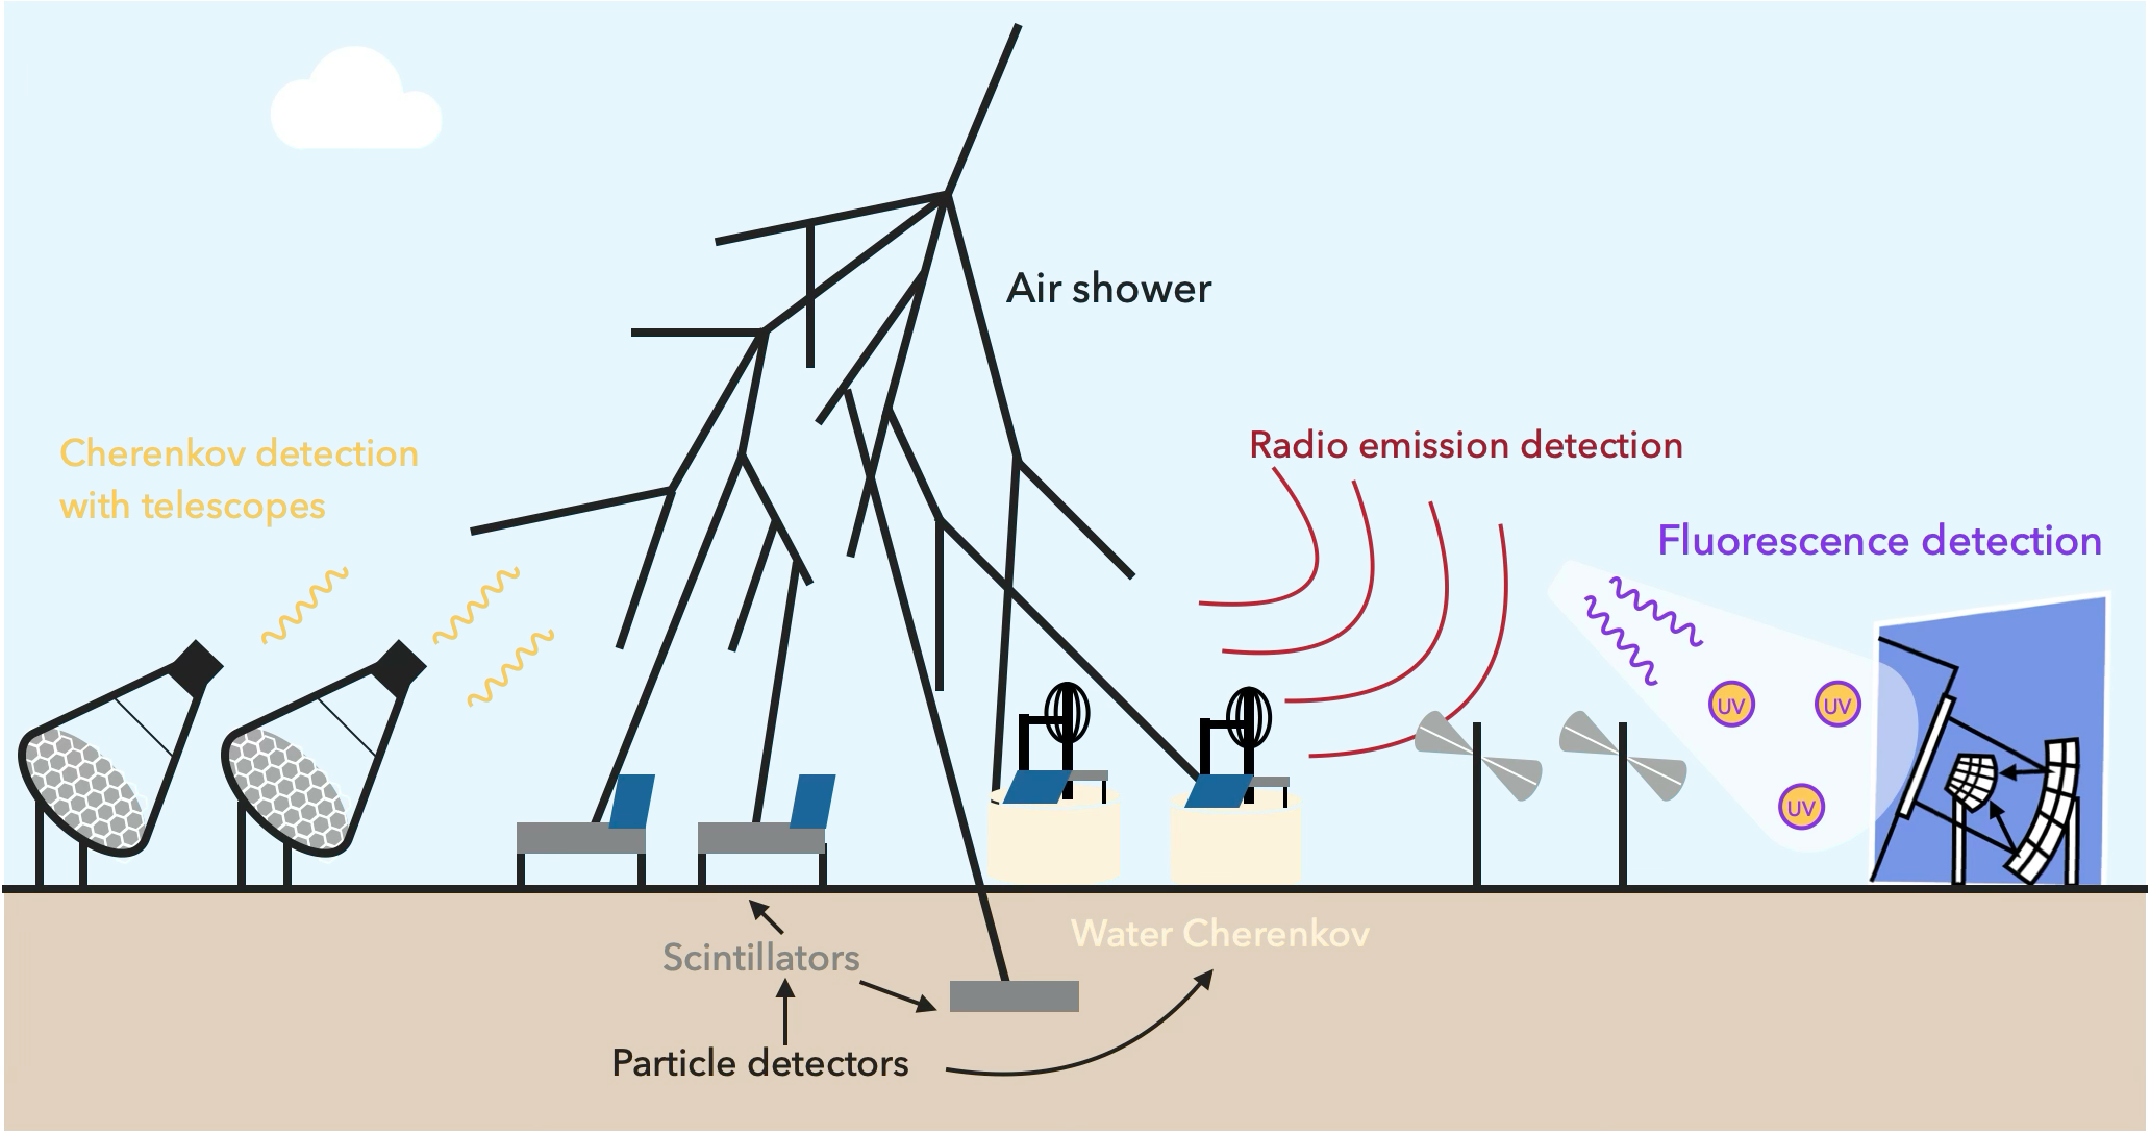
\includegraphics[width=14.5cm]{thesis_figures/EAS/EAS-Detection-Techniques-mine.pdf}
    \caption{Sketch of various ways to study experimentally extensive air showers. Inspired from~\cite{article_2001_kampert}} 
    \label{fig:EAS_det_techniques}
\end{figure}

\subsection{Radio Detection}
\label{sec:EAS_rad}
When an extensive air shower (EAS) travels through the atmosphere, it generates radio emissions primarily due to two mechanisms: the geomagnetic effect and the Askaryan effect. In air showers, the geomagnetic emission dominates, contributing around 85-90\% of the total signal, while the Askaryan effect accounts for the remaining 10-15\%~\cite{1966RSPSA.289..206K, Askaryan:1961pfb, osti_4100652}. The geomagnetic effect occurs when electrons and positrons in the shower are deflected by Earth's magnetic field, creating a dynamic current that moves at nearly the speed of light. This process generates a forward-focused radio signal with a lateral distribution described by the NKG relation.

The strength and characteristics of the radio signal depend on the geomagnetic field's orientation and atmospheric conditions at the detector site. At distances around 100 meters from the shower core, the detected frequencies are in the MHz range~\cite{Huege_2016}, while near the core, they extend into the GHz range. For primary energies above \(10^{17}\) eV, the emissions from both mechanisms overlap, with the measured electric field scaling directly with the shower's primary energy. This radio detection approach offers a valuable alternative to fluorescence and Cherenkov methods, free from the operational limitations of a restricted duty cycle.

Several radio antenna arrays are currently used for EAS detection, including LOFAR~\cite{2013A&A...556A...2V} and AERA~\cite{PhysRevD.93.122005}. The Pierre Auger Observatory is enhancing its capabilities by installing radio antennas on each unit of its particle detector array, expected to become fully operational by end of 2024. Future experiments, such as GRAND~\cite{fang2017giantradioarrayneutrino} and IceCube-Gen-2~\cite{Aartsen_2021_Gen-2}, aim to expand this field further. Additionally, observatories like RNO-G~\cite{Aguilar_2021} are also using this technique for neutrino detection. 


\subsection{Particle detector arrays}
\label{sec:EAS_particle}
This is one of the oldest detection techniques used to measure and study CRs. It consists of setting up a set of particle detectors (stations) spaced by large distances, depending on the desired energy range sensitivity of the experiment which is also dependent on the altitude of the experiment. The detectors are usually arranged in a regular pattern, and they are able to detect the secondary particles of EAS at ground by searching for time coincidences between neighbouring stations. By measuring the signal and time delay between the triggered stations the incoming direction of the primary can be estimated to $0.5^{\circ}-1^{\circ}$ of zenith angle resolution. The core position can also be determined by using the lateral distribution function (eq.~\ref{eq:Lateral_dist_func}) to fit the recorded signal at the surface detector array. The energy can also be estimated through the measurement of number of muons at ground or cross calibration with other detector systems. Different types of detection methods have been used to combine and act as particle detector arrays. These include Geiger counters at Harwell~\cite{1953Natur.171..349G}, hodoscopes at Kiel~\cite{1965ICRC....2..738B}, scintillators at Volcano ranch~\cite{Linsley1961485} and water or ice based Cherenkov detectors. Currently, scintillator based surface detector arrays and water or ice based Cherenkov tanks are the popularly used EAS detection techniques. 

Water/ice based Cherenkov tanks/detectors can also detect the secondary particles of EAS at ground. These are sensitive to the Cherenkov light which is produced by the charged particles while travelling through the medium of the detector. The subsequent light is measured using a photomultiplier tube (PMT). This light signature is different depending on the type of the particle and thus can effectively help in differentiating between muons and electrons. The Pierre Auger Observatory uses an array of water Cherenkov tanks in conjunction with five fluorescence detectors for EAS measurements. IceCube also contains an array of ice based Cherenkov detectors which are used for cosmic ray studies and as a veto for their underground neutrino detectors. More details about the Pierre Auger Observatory are presented in the next chapter~\ref{chap:setup}

Scintillator based particle detector arrays can be used to distinguish between the different secondary particles of an EAS. These consist of scintillating material which produces detectable photons if a charged particle traverses through the material. If deployed at the surface, such detectors can act as discriminators for electron and muons whereas if deployed underground they can only detect muons. The size of the scintillating material controls the zenith angle sensitivity which typically decreases as the inclination of the shower increases. TA uses a vast array of scintillator based detectors along with three fluorescence detectors to measure EAS. The Pierre Auger Observatory is also testing an array of underground muon detectors which are situated directly below its surface array stations.


\subsection{Towards detecting Neutrino Induced Extensive Air Showers}
\label{sec:EAS_nu}
Neutrino induced EASs can be differentiated from a regular CR induced EASs by their unique signature. Since neutrinos can interact at any atmospheric depth only the EASs that were initiated very deep in the atmosphere can be differentiated from a CR induced shower which typically starts at the top of the atmosphere. The deeper interaction means less shower development till the shower front reaches the ground in comparison to a cosmic ray induced EAS. This difference in development can be measured by the muon to electron ratio at ground via a particle detector array. Since, the neutrinos are only expected to interact and induce an EAS if the volume of the atmosphere through which they traverse is large enough. For zenith angles less than $60^{\circ}$ either the neutrinos are not expected to interact till they reach the ground and even if they do, due to the general amount of atmospheric volume at these angles the CR induced EASs are supposed to be indistinguishable from a neutrino shower, at least for a particle detector array at ground. This is due to the fact that the CR induced EASs have not developed enough to significantly reduce or lose their electromagnetic component. This leaves the primary distinguishing factor i.e. the muon to electron ratio the same for neutrino and CR induced EASs. The terminology used to determine the development of the shower in the atmosphere is the shower age and typically showers having a larger muonic component at ground are called \textit{old showers} while showers having a larger electromagnetic component at ground are called \textit{young showers}. 

Thus, to detect a neutrino induced EAS using surface detector arrays the smoking gun signal is an inclined ($\approx$ zenith angle > $60^{\circ}$) "young" shower. A perfect neutrino air shower detector should have a good angular resolution and a large electron-muon signal separation. However, this signature also not completely background free. Such a signature can also be caused by deeply interacting CR primaries or highly energetic muons emitting bremsstrahlung photons both of which can also induce a young shower at large zenith angles. B meson could also be misidentified as a neutrino as shown in~\cite{article_b_MESONS}. Other processes such as low energy showers coincident with an EAS could also act as background for a neutrino detection. These have been studied in detail in ~\cite{gap_note_2013} and are negated in the analysis through the techniques developed in the reference. 